\section{Source spectra, identifiability and finite-moment bounds}\label{sec:spectral}
\subsection{Physical sources and relative transfer moments}

Let $U_{\rm micro,\mathcal R}$ be the regulated microscopic update and $V_{\chi,\mathcal R}$ a proposed gauge-invariant source for a stable neutral state. With the reference-vacuum branch treated consistently, its relative transfer and moments are
\begin{equation}
W_{\chi,\mathcal R}=\overline U_{0,\mathcal R}\otimes U_{\chi,\mathcal R},\qquad
C_{n,\mathcal R}^{\chi}=V_{\chi,\mathcal R}^\dagger W_{\chi,\mathcal R}^{n}V_{\chi,\mathcal R},\quad C_0=I.
\end{equation}
A particle interpretation combines a positive-norm stable pole of the continued physical correlator with a dispersion relation in the common continuum state. Its rest energy gives $m_\chi=E_\chi(\mathbf 0)/c^2$ after temporal metrology and physical source normalization are fixed. Receiver neutrality specifies a symmetry label; the pole, stability and mass are dynamical properties.

Decay amplitudes follow from amputated three- or higher-point functions. Two-body annihilation and elastic scattering use connected, amputated four-point functions. Elastic nucleon scattering involves a matched composite source and the vertex $\Gamma^{(4)}_{\chi\chi NN}$. Thermal production is governed by the collision functional in the specified cosmological state.

\subsection{The information carried by finite moments}
\label{sec:moment}
A finite spectral certificate establishes positivity and consistency of the recorded moments. The following construction characterizes the spectral information retained by a truncated sequence.

\begin{proposition}[Non-unique spectral types for truncated moments]\label{prop:indeterminate}
For every positive integer $N$ there are two normalized positive spectral measures on the unit circle whose transfer moments agree for all $|n|\leq N$, although one is purely continuous and the other is purely atomic. The statement holds for normalized $6\times6$ matrix-valued transfer moments.
\end{proposition}
\begin{proof}
Let $\mu_{\rm H}=\dd\theta/(2\pi)$ be normalized Haar measure on the unit circle, and let $\mu_{\rm R}=(N+1)^{-1}\sum_{j=0}^{N}\delta_{\exp(2\pi i j/(N+1))}$ be the uniform measure on the $(N+1)$st roots of unity. Orthogonality of complex exponentials gives
\begin{equation}
\int z^n\,\dd\mu_{\rm H}(z)=\int z^n\,\dd\mu_{\rm R}(z)=0
\quad(1\leq |n|\leq N),\qquad
\int\dd\mu_{\rm H}=\int\dd\mu_{\rm R}=1.
\end{equation}
The former measure is continuous, while the latter has $N+1$ positive atoms, each of weight $1/(N+1)$. For six channels take $\dd\mathsf M=I_6\dd\mu$; this preserves normalized matrix positivity and exactly the same first $N$ moments. The associated unitary multiplication operators exist on their respective $L^2$ spaces. They have identical truncated Toeplitz moment matrices but different spectral types.\end{proof}

These measures establish that finite positivity alone permits distinct spectral types. Invariant-subspace and rank information identify particular finite sequences exactly, as proved in Section~\ref{sec:flat-reconstruction}. The continuum particle interpretation additionally refers to a common source family, physical energy branch and controlled regulator limit.

\begin{proposition}[Scale ambiguity of dimensionless spectral moments]\label{prop:scale}
With fixed dimensionless update matrices and transfer moments, rescaling the receiver time $\tau_*$ generates a corresponding family of physical energy spectra.
\end{proposition}
\begin{proof}
Write a unitary eigenphase as $\exp(-i\vartheta)$ and let a physical quasienergy be $E=(\hbar/\tau_*)\vartheta$ after the branch and physical continuation are specified. The map $\tau_*\mapsto s\tau_*$ with $s>0$ leaves all dimensionless powers of the update and the moments $V^\dagger W^nV$ unchanged while changing each energy to $E/s$. The same dimensionless data therefore represent a continuous family of dimensional energy scales.\end{proof}

The gravitational matching has the analogous dependence on metrology. Its common-state covariance is derived in Section~\ref{sec:metric}.

\label{sec:odd-no-go}
The stationary six-source C9 moments constrain the measure of their specified matter sources. Source visibility gives an exact characterization of the independent information in a copy-odd sector.
\begin{proposition}[Odd-sector non-identifiability when sources omit that sector]\label{prop:odd-nonidentification}
Let $\mathcal H_e$ be a Hilbert space carrying a unitary transfer $W_e$ and a collection of normalized source maps $V_f:\mathbb C^6\to\mathcal H_e$. Suppose the measured data consist of $C_n^{(f)}=V_f^\dagger W_e^nV_f$ for any finite or infinite set of integers $n$. These data admit unitary extensions with exactly the same source moments and an arbitrarily prescribed odd-sector eigenphase.
\end{proposition}
\begin{proof}
For every $\vartheta\in(-\pi,\pi]$, let $\mathcal H_\vartheta=\mathcal H_e\oplus\mathbb C$ and $W_\vartheta=W_e\oplus e^{-i\vartheta}$. Extend every source by zero, $\widetilde V_f u=(V_fu,0)$, and define the parity $P=I_{\mathcal H_e}\oplus(-1)$. Then $P$ commutes with $W_\vartheta$ and the odd one-dimensional summand has unitary eigenvalue $e^{-i\vartheta}$, yet
\[
\widetilde V_f^\dagger W_\vartheta^n\widetilde V_f=V_f^\dagger W_e^nV_f
\quad\text{for every }f,n.
\]
The entire set of moments supported in $\mathcal H_e$, including all orders and all positive Toeplitz tests, remains unchanged as $\vartheta$ varies. The odd-sector phase, its dispersion and physical clock define additional data for the mass prescription. The construction concerns the specified source moments; a fully specified microscopic update fixes its own sector dynamics.
\end{proof}
With an odd source included, the spectral information is described by its own matrix moment problem. A positive atomic lower weight together with a gap establishes a visible isolated spectral component. The inverse-Toeplitz result derived below supplies an upper weight compatible with the recorded moments. Spin, helicity and the physical continuum interpretation belong to the corresponding source and symmetry structure.

For a normalized source whose range defines the first block, the projected resolvent has the exact form
\begin{equation}
G_\chi(z)=V_\chi^\dagger(z-W_\chi)^{-1}V_\chi
=\big[z-A_\chi-B_\chi(z-D_\chi)^{-1}C_\chi\big]^{-1}
\label{eq:odd-feshbach}
\end{equation}
for $W_\chi=\bigl[\begin{smallmatrix}A_\chi&B_\chi\\ C_\chi&D_\chi\end{smallmatrix}\bigr]$ and $z\in\rho(W_\chi)\cap\rho(D_\chi)$. The two off-diagonal blocks are independent blocks of a unitary operator. The Feshbach--Schur identity follows by eliminating the second block in $(z-W_\chi)X=V_\chi$. Its poles and residues characterize the finite source resolvent; an isolated physical branch additionally satisfies the common continuum and metrological prescription.

\subsection{Exact grading and stability}
\label{sec:operator-route}

An exact copy-opposition grading supplies a selection rule when it commutes with the full interacting update. Stability combines this symmetry with the physical energy thresholds of all allowed final states.

\begin{proposition}[Copy parity and the decay threshold]\label{prop:copy-odd}
Let $P_{\rm cp}=P_{\rm cp}^\dagger$, $P_{\rm cp}^2=I$ and $[U,P_{\rm cp}]=0$ on the physical Hilbert space. Transfer matrix elements between opposite parities vanish for all integer times. Suppose also that a positive physical Hamiltonian conserves parity and energy, and that an odd one-particle branch $\chi$ exists with rest energy $m_\chi c^2$. If every multiparticle final state with the same conserved charges and odd parity has threshold strictly above $m_\chi c^2$, then $\chi$ is stable against decay into those states. The threshold is taken over the complete physical sector, including gauge-invariant combinations of charged particles.
\end{proposition}
\begin{proof}
Insertion of the commuting parity on both sides gives
$\langle\psi_+|U^n|\psi_-\rangle=-\langle\psi_+|U^n|\psi_-\rangle$, so the matrix element vanishes. Thus every allowed final state has odd total parity. By the stated threshold hypothesis, each such multiparticle state has energy greater than the rest energy of $\chi$, and energy conservation forbids the decay. A lightest odd particle together with a strictly positive gap to every additional allowed daughter satisfies this condition. Channels at an equal threshold, including infrared dressing by massless fields, are governed by their separate pole and scattering assumptions.
\end{proof}

For copy-even visible matter, the exact effective action contains even powers of an odd field. Parity permits quadratic portal interactions, including the four-point nucleon-scattering vertex. The source-visible branch, its thresholds and the same-state connected vertex are the corresponding physical inputs.

\subsection{Energy branches and interaction data}
\label{sec:energy-vertices}
A fixed clock converts a selected phase branch into an energy. The branch itself carries independent information even when the complete one-step transfer is known.
\begin{proposition}[Energy branches of a unitary transfer]\label{prop:energy-branch}
For a finite unitary $W=\sum_j e^{-i\theta_j}\Pi_j$ and fixed $\tau_*>0$, every integer choice $n_j$ defines a self-adjoint generator
\begin{equation}\label{eq:energy-branch}
H_{\boldsymbol n}=\frac{\hbar}{\tau_*}\sum_j(\theta_j+2\pi n_j)\Pi_j,
\qquad e^{-i\tau_*H_{\boldsymbol n}/\hbar}=W.
\end{equation}
Infinitely many such generators are positive. Specifying an admissible energy interval of width less than $2\pi\hbar/\tau_*$ selects at most one representative for each phase.
\end{proposition}
\begin{proof}
The exponential removes every integer multiple of $2\pi$. Choosing sufficiently large integers makes all eigenvalues positive. Two representatives of the same phase differ by an integer multiple of $2\pi\hbar/\tau_*$, so an interval shorter than this spacing contains at most one. Existence also requires that the stated interval contain a representative of every relevant phase.
\end{proof}
The physical particle prescription therefore combines source visibility, an energy branch, momentum dispersion and clock normalization. Positivity alone leaves the displayed family of energy branches admissible.

\begin{proposition}[Independent interaction content at fixed two-point spectrum]\label{prop:interaction-data}
Normalized vacuum-to-one-particle transfer moments can remain identical while connected four-point functions vary in an exactly parity-conserving, positive-energy family.
\end{proposition}
\begin{proof}
In units $\hbar=1$, take a bosonic mode with number operator $\widehat N$, vacuum $|0\rangle$, and
\[
H_g=\omega\widehat N+\frac g2\widehat N(\widehat N-1),\qquad
\omega>0,\quad g\geq0,\quad P=(-1)^{\widehat N}.
\]
Each Hamiltonian is positive and commutes with $P$. For the normalized odd source $a^\dagger|0\rangle=|1\rangle$, every transfer moment equals $e^{-in\tau_*\omega}$, independently of $g$. In contrast, the two-particle propagation and its connected part are
\begin{align}
\langle0|a^2e^{-itH_g}(a^\dagger)^2|0\rangle&=2e^{-it(2\omega+g)},\\
G^{(4)}_{\rm conn}(t)&=2e^{-2it\omega}(e^{-igt}-1).
\end{align}
The second expression follows by subtracting the two vacuum pair contractions. Its dependence on $g$ proves the assertion.
\end{proof}
This algebraic example identifies the independent role of multiparticle dynamics. In a relativistic particle model, the connected correlator, its physical continuation and external-state normalization determine the amputated amplitude. The portal couplings in Section~\ref{sec:thermal} specify this interaction information for that effective model.

\subsection{Positive matrix bounds on spectral weight}
\label{sec:fejer-certificate}
\begin{proposition}[Fej\'er upper bound on atomic matrix weight]\label{prop:fejer}
Let $W$ be unitary and $V$ an isometry from a $d$-dimensional source space. Let $C_n=V^\dagger W^nV=\int_{-\pi}^{\pi}e^{in\varphi}\,\mathrm d\mu(\varphi)$, $C_0=I_d$. Given the first $N$ nonnegative moments, set
\begin{equation}
F_N(\theta)=\frac1{N^2}\left[N C_0+\sum_{k=1}^{N-1}(N-k)\left(e^{-ik\theta}C_k+e^{ik\theta}C_k^\dagger\right)\right].\label{eq:fejer-matrix}
\end{equation}
For every $\theta$, the matrix-valued atom $M_\theta:=\mu(\{\theta\})$ satisfies
\begin{equation}\label{eq:fejer-order}
\boxed{0\preceq M_\theta\preceq F_N(\theta)\preceq I_d.}
\end{equation}
If all other spectral support is separated from $\theta$ by an angular distance at least $\Delta>0$, let $q_N=\min\{1,[N^2\sin^2(\Delta/2)]^{-1}\}$. When $q_N<1$, the complementary lower bound is
\begin{equation}
M_\theta\succeq\frac{F_N(\theta)-q_NI_d}{1-q_N}.
\label{eq:fejer-gap-lower}
\end{equation}
\end{proposition}
\begin{proof}
The spectral theorem gives the positive integral representation
\begin{equation}
F_N(\theta)=\int\left|\frac1N\sum_{j=0}^{N-1}e^{ij(\varphi-\theta)}\right|^2\mathrm d\mu(\varphi).
\end{equation}
The scalar integrand belongs to $[0,1]$ and equals one at $\varphi=\theta$. The atom therefore contributes precisely $M_\theta$, with a remaining positive matrix contribution bounded by $I_d-M_\theta$, giving Eq.~\eqref{eq:fejer-order}. Away from an isolated atom by at least $\Delta$, the geometric-sum formula bounds the integrand by $[N^2\sin^2(\Delta/2)]^{-1}$. Thus $F_N\preceq M_\theta+q_N(I_d-M_\theta)$; rearrangement proves Eq.~\eqref{eq:fejer-gap-lower}. The lower enclosure uses the asserted gap as an explicit hypothesis.
\end{proof}

\begin{proposition}[Inverse-Toeplitz upper bound for a matrix atom]\label{prop:christoffel}
Let $C_k=\int z^k\,\mathrm d\mu(z)$, $C_0=I_d$, and let
\begin{equation}
T_N=[C_{j-k}]_{j,k=0}^{N-1},\qquad C_{-k}=C_k^\dagger,
\quad A_N(\theta)=\begin{bmatrix}I_d&e^{i\theta}I_d&\cdots&e^{i(N-1)\theta}I_d\end{bmatrix}^{\!\mathsf T}.
\end{equation}
If $T_N$ is strictly positive definite, the matrix spectral atom $M_\theta=\mu(\{e^{i\theta}\})$ obeys
\begin{equation}\label{eq:christoffel-bound}
\boxed{0\preceq M_\theta\preceq B_N(\theta):=
\left[A_N(\theta)^\dagger T_N^{-1}A_N(\theta)\right]^{-1}.}
\end{equation}
Moreover $B_N(\theta)\preceq F_N(\theta)$, where $F_N$ is the normalized Fej\'er bound of Proposition~\ref{prop:fejer}.
\end{proposition}
\begin{proof}
The spectral integral of $v_N(z)=[I_d,zI_d,\ldots,z^{N-1}I_d]^\mathsf T$ implies $T_N\succeq A_NM_\theta A_N^\dagger$. This form applies directly even when the atomic weight is singular. For every block column $L$ satisfying $A_N^\dagger L=I_d$, multiplication gives $M_\theta\preceq L^\dagger T_NL$. The minimum is attained at $L_*=T_N^{-1}A_N(A_N^\dagger T_N^{-1}A_N)^{-1}$, because the cross terms vanish for every perturbation $Q$ with $A_N^\dagger Q=0$. The uniform choice $L=A_N/N$ yields $F_N$, proving $B_N\preceq F_N$.\end{proof}

The bound has a directly usable perturbation form. If an approximate Hermitian Toeplitz matrix $\widehat T_N$ obeys $\|T_N-\widehat T_N\|_2\leq\varepsilon$ and $\widehat T_N+\varepsilon I\succ0$, then
\begin{equation}\label{eq:christoffel-robust}
M_\theta\preceq \left[A_N^\dagger(\widehat T_N+\varepsilon I)^{-1}A_N\right]^{-1}.
\end{equation}
Indeed $A_NM_\theta A_N^\dagger\preceq T_N\preceq\widehat T_N+\varepsilon I$. For separately verified moment errors $\|\Delta C_k\|_2\leq\delta_k$, one may take $\varepsilon=\delta_0+2\sum_{k=1}^{N-1}\delta_k$. The tabulated nominal values use the stored moments as given; physical continuum applications additionally specify verified $\delta_k$. Equation~\eqref{eq:christoffel-robust} propagates such verified errors into the atomic-weight enclosure.

The optimized bound uses all moment covariances and assumes positivity of the Toeplitz matrix. A floating-point evaluation estimates the bound for the recorded moments; the rational calculation below gives an exact enclosure for an explicitly normalized version of those data. Physical source and regulator errors enter through the stated perturbation bounds.

\paragraph{Direct evaluation using the supplied QICT moments.}
The supplied stationary C9 moment data contain thirteen complex $6\times6$ moments for each of four finite stationary C9 regulators. Direct evaluation of Eq.~\eqref{eq:fejer-matrix} at $\theta=0$ gives the following eigenvalue ranges; all rows have $\|C_0-I_6\|_F<2.5\times10^{-14}$.

\begin{table}[ht]
\centering\small
\caption{Matrix-Fej\'er upper bounds for the stationary six-source C9 measure at $z=1$. The entries constrain atomic weight in the specified finite matter-source measure.}
\begin{tabular}{@{}lrrr@{}}\toprule
Regulator & Neutral dimension & $\lambda_{\min}(F_{13}(0))$ & $\lambda_{\max}(F_{13}(0))$\\\midrule
R1 & 45 & 0.001564899 & 0.016935575\\
R2 & 350 & 0.001411760 & 0.015844046\\
R3 & 1470 & 0.001430216 & 0.016046359\\
R4 & 4455 & 0.001430296 & 0.016083559\\
\bottomrule\end{tabular}\label{tab:fejer-qict}
\end{table}

\begin{figure}[ht]
\centering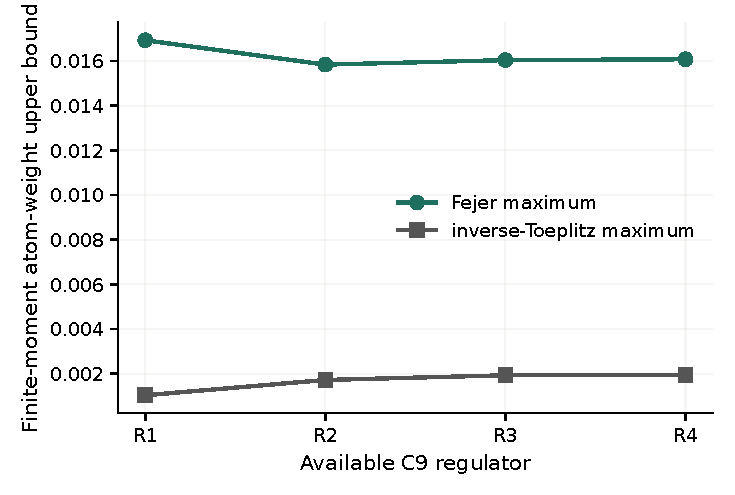
\includegraphics[width=.76\linewidth]{figures/spectral_atom_bounds.pdf}
\caption{Fej\'er and optimized inverse-Toeplitz bounds from thirteen stationary C9 moments. Both concern the same six source channels on finite regulators.}\label{fig:fejer-qict}
\end{figure}

For the full $13\times13$ block Toeplitz matrices, all four input sets are numerically positive definite. Their inverse-Toeplitz atom bounds are

\begin{table}[ht]
\centering\small
\caption{Optimized matrix-polynomial upper bounds $B_{13}(0)$, evaluated from the same thirteen stationary C9 moments. The improvement is relative to the Fej\'er maximum eigenvalue and carries the same finite-source interpretation.}\label{tab:christoffel-qict}
\begin{tabular}{@{}lrrr@{}}\toprule
Regulator & $\lambda_{\min}(B_{13})$ & $\lambda_{\max}(B_{13})$ & Fej\'er / optimized ratio\\\midrule
R1 & 0.0000507384 & 0.0010364794 & 16.34\\
R2 & 0.0000770880 & 0.0017207756 & 9.21\\
R3 & 0.0000773188 & 0.0019325137 & 8.30\\
R4 & 0.0000773178 & 0.0019562730 & 8.22\\
\bottomrule\end{tabular}
\end{table}

At R4, every eigenvalue of the zero-phase atomic weight is bounded by $0.0019562731$ in the nominal floating-point calculation, compared with the Fej\'er bound $0.0160835595$. The stored results include each $13$-block linear-solve residual and smallest Toeplitz eigenvalue. The $5\times5$ block tests give minimum eigenvalues approximately $2.68\times10^{-4}$, $4.78\times10^{-4}$, $5.03\times10^{-4}$ and $5.05\times10^{-4}$ for R1--R4. These are properties of the supplied six C9 matter-source channels. A transverse-traceless metric source defines a distinct spectral measure, to which the same mathematical bounds apply with its own moments and physical normalization.


\subsection{Finite identification, source visibility and the cyclic domain}
The truncated-moment example in Proposition~\ref{prop:indeterminate} establishes non-uniqueness for a class of admissible data. Particular finite moment sequences can identify a spectrum exactly. The appropriate distinction is between generic positive moment information and additional rank or invariance information.
\begin{proposition}[An exactly identifiable finite case]\label{prop:unitary-first-moment}
Let $W$ be unitary, $V^\dagger V=I_d$, and $C_1=V^\dagger WV$. If $C_1$ is unitary, then $WV=VC_1$, the source range reduces $W$, and $C_n=C_1^n$ for every integer $n$. Its source spectral measure is exactly the spectral measure of $C_1$.
\end{proposition}
\begin{proof}
The orthogonal component satisfies
\[
[(I-VV^\dagger)WV]^\dagger[(I-VV^\dagger)WV]=I-C_1^\dagger C_1=0.
\]
Thus $WV=VC_1$. Unitarity of $C_1$ makes the finite source range invariant under both $W$ and $W^\dagger$, giving the assertion by iteration. For example, $C_1=I_d$ fixes the source measure to $I_d\delta_1$.
\end{proof}
More generally, all source moments determine the unitary dynamics on the reducing cyclic subspace
\[
\mathcal K=\overline{\operatorname{span}}\{W^nVu:n\in\mathbb Z,\ u\in\mathbb C^d\}.
\]
Indeed, the moments determine every inner product between the displayed generating vectors. Two realizations with the same moments therefore have an isometric identification of their dense cyclic spans, extending to a unitary intertwiner on $\mathcal K$. Dynamics on $\mathcal K^\perp$ remain independent of the recorded source data. Proposition~\ref{prop:odd-nonidentification} is the parity-resolved instance of this source-visibility statement. Physical particle identification additionally specifies the energy branch, momentum dispersion and continuum state.

\subsection{Finite reconstruction from a stable moment rank}
\label{sec:flat-reconstruction}
The unitary-first-moment criterion extends to a source space generated by several transfer steps. In this setting, a stable Gram rank gives a finite reconstruction of the entire visible dynamics.
\begin{proposition}[Flat-rank reconstruction]\label{prop:flat-rank}
Let $C_0=I_d$ and suppose that the positive block Toeplitz matrix $T_{N+1}$ satisfies
\[
\operatorname{rank}T_{N+1}=\operatorname{rank}T_N=r.
\]
Then every unitary realization of these moments has the same $r$-dimensional cyclic source dynamics up to unitary equivalence. Its source measure is a finite sum of at most $r$ atoms, and the recorded moments determine all subsequent moments.
\end{proposition}
\begin{proof}
In a unitary realization define $\mathcal K_N=\operatorname{span}\{W^{-j}Vu:0\leq j<N\}$. The Gram matrix of these vectors is $T_N$. Equality of the two ranks therefore gives $\mathcal K_{N+1}=\mathcal K_N$. In particular, $W^{-1}\mathcal K_N\subseteq\mathcal K_N$. The restriction of $W^{-1}$ is an isometry of a finite-dimensional space onto itself, so $\mathcal K_N$ reduces $W$ and equals the full cyclic source space.

For an explicit reconstruction, factor $T_N=S^\dagger S$ with $S$ of full row rank $r$. Write $S^+$ for its Moore--Penrose inverse and form
\[
H_N=[C_{j-k-1}]_{j,k=0}^{N-1},\qquad
U_-=(S^+)^\dagger H_NS^+,\qquad Q=S_{[:,1:d]}.
\]
The columns of $S$ are coordinates of the source generators, while $H_N$ contains their inner products with the shifted generators. Thus $U_-$ represents $W^{-1}|_{\mathcal K_N}$ and is unitary. Every moment is
\begin{equation}\label{eq:flat-reconstruction}
C_n=Q^\dagger(U_-^\dagger)^nQ,\qquad n\in\mathbb Z.
\end{equation}
Diagonalization of $U_-^\dagger$ gives the phases and the positive matrix residues $Q^\dagger\Pi_jQ$, whose sum is $I_d$. A different full-row-rank Gram factor changes these coordinates by a unitary transformation and preserves the measure.
\end{proof}
For the normalized recorded C9 data, the exact positivity of $T_{13}$ gives $\operatorname{rank}T_{13}=78$, whereas $\operatorname{rank}T_{12}=72$. The supplied sequence therefore remains in the growing-rank regime. Its minimal cyclic realization has dimension at least 78. The independent reconstruction test uses a seven-dimensional unitary with two sources: $\operatorname{rank}T_4=\operatorname{rank}T_5=7$, and the recovered operator reproduces moments through order 21 to an operator-norm discrepancy below $2.5\times10^{-14}$. This test illustrates the exact rank criterion with explicitly declared finite matrices.

\subsection{Quantitative control near an invariant source space}
\begin{proposition}[Source-leakage bound]\label{prop:source-leakage}
Let $C_n=V^\dagger W^nV$, with $W$ unitary and $V$ a finite-dimensional isometry. Set $\varepsilon=\|I-C_1^\dagger C_1\|_2$. For every integer $n\geq1$,
\begin{equation}\label{eq:source-leakage}
\|C_n-C_1^n\|_2\leq\min\{2,\tfrac12n(n-1)\varepsilon\}.
\end{equation}
\end{proposition}
\begin{proof}
Write $P=VV^\dagger$. The two off-diagonal couplings obey
\[
\|(I-P)WV\|_2^2=\|I-C_1^\dagger C_1\|_2=\varepsilon,
\qquad \|V^\dagger W(I-P)\|_2^2=\|I-C_1C_1^\dagger\|_2=\varepsilon.
\]
The last equality follows from the common singular values of the square matrix $C_1$. Iterating the complementary-space equation gives $\|(I-P)W^kV\|_2\leq k\sqrt\varepsilon$, since both compressed blocks are contractions. Now
\[
C_{k+1}=C_1C_k+V^\dagger W(I-P)W^kV.
\]
Successive substitution bounds the difference from $C_1^n$ by $\sum_{k=1}^{n-1}k\varepsilon$. Both terms are contractions, which also gives the bound two.
\end{proof}
The estimate quantifies how accurately powers of the first moment represent the true moments over a finite transfer interval. Its exact zero-leakage case is Proposition~\ref{prop:unitary-first-moment}.

\subsection{Optimality and monotonicity of the Toeplitz bound}
The optimized bound is a matrix counterpart of the classical Christoffel extremal problem \cite{Simon05}. The following argument establishes its exact truncated-moment characterization directly.
\begin{proposition}[Feasible atomic weights and nested information]\label{prop:sharp}
Suppose $T_N\succ0$ and let $A=A_N(\theta)$. A positive component $M\delta_{e^{i\theta}}$ can be included in a positive matrix measure with the recorded moments if and only if
\[
T_N-AMA^\dagger\succeq0.
\]
The largest feasible component is the exact atomic weight $B_N(\theta)$ in an extremal representing measure, and, for compatible strictly positive successive moment matrices,
\begin{equation}\label{eq:nested-bounds}
0\preceq M_\theta\preceq B_{N+1}(\theta)\preceq B_N(\theta)\preceq F_N(\theta).
\end{equation}
\end{proposition}
\begin{proof}
Subtracting the proposed atom leaves the block Toeplitz matrix of the residual moments. A positive block Toeplitz matrix admits a positive matrix-valued representing measure: factor its Gram form, identify the shift between equal-length overlapping polynomial spans, and extend that isometry to a unitary after an auxiliary-space completion. Its spectral resolution supplies the residual measure. Adding the proposed atom recovers the original moments. Necessity follows directly by integrating its positive contribution.

For the maximal bound define $L_*=T_N^{-1}A(A^\dagger T_N^{-1}A)^{-1}$. It satisfies $A^\dagger L_*=I_d$. Every other $L$ satisfying this constraint can be written $L=L_*+Q$, $A^\dagger Q=0$, whence
\[
L^\dagger T_NL=B_N+Q^\dagger T_NQ\succeq B_N.
\]
Equivalently, $T_N-AB_NA^\dagger\succeq0$, and $AMA^\dagger\preceq T_N$ implies $M\preceq B_N$ by multiplication with $L_*^\dagger,L_*$. At this maximum the residual measure has zero additional atom at $e^{i\theta}$, since any positive additional weight would violate the upper bound. Increasing $N$ restricts the feasible set; alternatively, append a zero coefficient to any lower-degree polynomial. This proves monotonicity. The uniform polynomial gives $F_N$.
\end{proof}
For singular $T_N$, direct inversion is replaced by the exact conditions
\[
\operatorname{ran}(AM^{1/2})\subseteq\operatorname{ran}T_N,
\qquad M^{1/2}A^\dagger T_N^+AM^{1/2}\preceq I_d,
\]
where $T_N^+$ is the Moore--Penrose inverse. These follow by factoring through $T_N^{1/2}$ on its range. They cover finitely identifiable singular cases without applying a positive-definite inverse outside its domain.

\subsection{Finite-resolution spectral weight and controlled moment errors}
For $N\geq2$, let $I_{\theta,\delta}$ be the circular arc within distance $\delta$ of $\theta$, with $0<\delta<\pi/(N-1)$. Centering the phases in the Fej\'er polynomial gives
\[
\left|\frac1N\sum_{j=0}^{N-1}e^{ijt}\right|^2
\geq\cos^2\!\left(\frac{(N-1)\delta}{2}\right)=:a_{N,\delta}>0
\quad (|t|\leq\delta).
\]
Each centered cosine is at least $\cos((N-1)\delta/2)$; summing proves the inequality. Positivity then yields the finite-resolution bound
\begin{equation}\label{eq:arc-bound}
0\preceq\mu(I_{\theta,\delta})\preceq a_{N,\delta}^{-1}F_N(\theta).
\end{equation}
Equation~\eqref{eq:arc-bound} constrains the total weight of an unresolved narrow feature. Its positive lower enclosures are given by additional support hypotheses, as in Proposition~\ref{prop:exponential-gap}.

For verified moment errors $\|C_k-\widehat C_k\|\leq\delta_k$, a more flexible certificate uses fixed polynomial coefficients $L_j$ satisfying $\sum_j e^{-ij\theta}L_j=I_d$. Its exact quadratic form and error budget are
\begin{equation}\label{eq:polynomial-error}
M_\theta\preceq L^\dagger T_N L
\preceq L^\dagger\widehat T_NL+\mathcal E_LI_d,\qquad
\mathcal E_L=\sum_{j,k=0}^{N-1}\delta_{|j-k|}\|L_j\|\|L_k\|.
\end{equation}
The first inequality follows from $T_N\succeq AM_\theta A^\dagger$; the second follows term by term from the operator norm inequality. Unlike an inverse perturbation estimate, this certificate can be checked using a proposed polynomial without certifying a numerical inverse.

\subsection{An exact rational certificate for the recorded C9 data}
All supplied $6\times6$ moments are diagonal, with three identical left-source entries and three identical right-source entries. We retain every input array unchanged and define a precisely normalized recorded moment problem by
\[
\widetilde C_0=I_6,\qquad
\widetilde C_k=S^{-1/2}C_kS^{-1/2}\ (k\geq1),\qquad
S=\operatorname{Re}C_0.
\]
The maximum normalization change in the input is of order $2.5\times10^{-14}$. The rational implementation interprets each stored binary number exactly, removes the tiny imaginary diagonal of $C_0$, and divides each scalar diagonal sequence by its positive real zeroth moment. It proves positivity by exact $13$-step $LDL^\dagger$ factorization in each of the eight distinct scalar blocks. A numerical solve proposes coefficients; exact rational arithmetic enforces their sum to one and evaluates their polynomial energy. The final outward-rounded upper bounds are

\begin{table}[htbp]\centering\small
\caption{Exact-rational polynomial bounds for the explicitly normalized recorded finite moment problem. Independent physical moment and continuum errors enter through Eq.~\eqref{eq:polynomial-error}.}
\begin{tabular}{@{}lrr@{}}\toprule
Regulator & Left-source upper weight & Right-source upper weight\\\midrule
R1 & 0.001036479358 & 0.000050738373\\
R2 & 0.001720775586 & 0.000077087987\\
R3 & 0.001932513690 & 0.000077318759\\
R4 & 0.001956273015 & 0.000077317777\\
\bottomrule
\end{tabular}\label{tab:exact-rational}
\end{table}

The polynomial certificate is exact for this finite recorded-data problem. The full interacting QICT source family and its regulator limit retain their separate physical error budget. This distinction makes the arithmetic guarantee explicit while preserving the physical interpretation of the six matter-source channels.

\subsection{Convergence of the optimal atomic-weight hierarchy}
\begin{proposition}[Recovery of a source-visible atom]\label{prop:atom-limit}
For one fixed normalized matrix spectral measure with strictly positive $T_N$ at every order,
\[
B_N(\theta)\downarrow\mu(\{e^{i\theta}\})\quad\text{as }N\to\infty.
\]
If all remaining support is separated by an angular gap $\Delta$, then
\[
0\preceq B_N(\theta)-M_\theta\preceq q_N(I_d-M_\theta),
\qquad q_N=\min\{1,[N^2\sin^2(\Delta/2)]^{-1}\}.
\]
\end{proposition}
\begin{proof}
The normalized Fej\'er integrand tends pointwise to one at the specified phase and to zero at every other phase, and is bounded by one. Dominated convergence for the finite positive trace measure gives $F_N\to M_\theta$ in the finite source dimension. The inequalities $M_\theta\preceq B_N\preceq F_N$, together with monotonicity, prove the first claim. The gap estimate in Proposition~\ref{prop:fejer} gives the stated quantitative squeeze.
\end{proof}
This limit concerns a fixed measure. The uniform-gap statement below gives an explicit sufficient condition for a joint regulator and moment limit.

\subsection{Exponential bounds under a certified angular gap}
\label{sec:gap-filter}
An angular gap permits a sharper polynomial filter than the uniform Fej\'er average. Let $0<\Delta<\pi$, $c_\Delta=\cos(\Delta/2)$ and $m=N-1\geq1$. Denote the Chebyshev polynomial of the first kind by $\mathsf T_m$. Define ordinary polynomials by
\[
P_0(z)=1,\quad P_1(z)=\frac{1+z}{2c_\Delta},\quad
P_{m+1}(z)=\frac{1+z}{c_\Delta}P_m(z)-zP_{m-1}(z),
\qquad p_m(z)=\frac{P_m(z)}{\mathsf T_m(c_\Delta^{-1})}.
\]
The recurrence gives $p_m(1)=1$. For a specified phase $\theta$, set
\[
Q_{m,\Delta}(\theta)=\int|p_m(e^{i(\varphi-\theta)})|^2\,\dd\mu(\varphi),
\qquad
q_{m,\Delta}=\operatorname{sech}^2\!\left[m\operatorname{arcosh}(c_\Delta^{-1})\right].
\]
The quadratic form $Q_{m,\Delta}$ uses only $C_0,\ldots,C_m$.
\begin{proposition}[Exponential enclosure of an isolated atom]\label{prop:exponential-gap}
If the support outside $e^{i\theta}$ lies at circular distance at least $\Delta$, then
\begin{equation}\label{eq:exponential-gap}
\frac{Q_{m,\Delta}-q_{m,\Delta}I_d}{1-q_{m,\Delta}}
\preceq M_\theta\preceq B_{m+1}(\theta)\preceq Q_{m,\Delta},
\end{equation}
where $B_{m+1}$ is defined when $T_{m+1}\succ0$. In particular,
\begin{equation}\label{eq:exponential-convergence}
0\preceq B_{m+1}(\theta)-M_\theta
\preceq q_{m,\Delta}(I_d-M_\theta),\qquad
q_{m,\Delta}\leq4e^{-2m\operatorname{arcosh}(c_\Delta^{-1})}.
\end{equation}
\end{proposition}
\begin{proof}
On the unit circle the recurrence gives
\[
P_m(e^{it})=e^{imt/2}\mathsf T_m\!\left(\frac{\cos(t/2)}{c_\Delta}\right).
\]
For $\Delta\leq|t|\leq\pi$, the argument lies in $[0,1]$, where $|\mathsf T_m|\leq1$. At $t=0$, the normalized modulus equals one. Over the intervening arc it is at most one because $\mathsf T_m(x)=\cosh(m\operatorname{arcosh}x)$ is increasing for $x\geq1$. Consequently
\[
M_\theta\preceq Q_{m,\Delta}\preceq M_\theta+q_{m,\Delta}(I_d-M_\theta).
\]
The polynomial extremal characterization gives $B_{m+1}\preceq Q_{m,\Delta}$. Rearrangement and $\cosh x\geq e^x/2$ establish both claims.
\end{proof}
For a known gap $\Delta=0.55$ and thirteen moments, the exponential remainder factor is $0.00498661$, compared with $0.0802460$ for the uniform-polynomial gap bound. These numbers refer to the stated gap hypothesis. The C9 upper bounds in Tables~\ref{tab:fejer-qict}--\ref{tab:exact-rational} retain their direct finite-moment interpretation.

The same estimate controls a simultaneous regulator limit. Suppose normalized measures $\mu_{\mathcal R}$ converge weakly to $\mu$, all have the same fixed phase and excluded punctured arc of width $\Delta$, and their moment matrices at the required orders are positive definite. A continuous function equal to one at $\theta$ and zero outside that arc gives $M_{\theta,\mathcal R}\to M_\theta$. Equation~\eqref{eq:exponential-convergence} then yields
\[
\|B_{N,\mathcal R}(\theta)-M_\theta\|_2
\leq q_{N-1,\Delta}+\|M_{\theta,\mathcal R}-M_\theta\|_2.
\]
Thus both orders of the regulator and moment limits recover the same atom under the stated uniform gap and weak-convergence assumptions. Verified moment errors are added through Eq.~\eqref{eq:polynomial-error}.
